\documentclass[aps, reprint,amsmath,amssymb]{revtex4-1} %APS Journal
\usepackage[T1]{fontenc}
\usepackage[utf8]{inputenc}
\usepackage{lmodern}
\usepackage{microtype}
\usepackage{graphicx}
\usepackage{siunitx}
\usepackage{bm}

\renewcommand{\vec}[1]{\boldsymbol{#1}}
\newcommand{\mat}[1]{\mathbf{#1}}
\newcommand{\uv}[1]{\vec{\hat{#1}}}
\newcommand{\x}{\vec{\hat{x}}}
\newcommand{\y}{\vec{\hat{y}}}
\newcommand{\z}{\vec{\hat{z}}}
\renewcommand{\d}{\partial}
\renewcommand{\L}{\mathcal{L}}
\renewcommand{\inf}{\infty}

\begin{document}
%----------------------------------------------------------------------
% title
%----------------------------------------------------------------------
\title{PHY64 Experiment 1: The Cavendish Experiment}
\author{Matthew S. E. Peterson}
\author{Jackson Burzynski}
\affiliation{Department of Physics and Astronomy\\Tufts University}
%\date{\today} 
\maketitle

%----------------------------------------------------------------------
% Body
%----------------------------------------------------------------------
\section{Introduction}

In 1797, British scientist Henry Cavendish became the first person to
successfully measure the gravitational interaction between two bodies in a
laboratory. The apparatus used by Cavendish consisted of a torsion balance
with two small lead spheres attached to either end, and two larger lead
spheres positioned on alternate sides of the horizontal arm of the balance.
By reflecting a light beam off of a mirror attached to the pendulum and
observing the change of position of the reflected beam on a distant
surface, Cavendish was able to observe a small difference in the
equilibrium position of the pendulum with the larger masses in place. Using
this method, Cavendish was successfully able to calculate Newton's
gravitational constant $G$ within $1\%$ of the currently accepted value. 

In this experiment, we replicate Cavendish's experiment using the
TEL-Atomic torsion pendulum that mimics the experimental setup used in
1797. The TEL-Atomic apparatus allows us to observe the oscillations of the
pendulum by way of an oscillating voltage readout on a computer. Using the
same technique as Cavendish did, we then calibrate the oscillations in
voltage to the pendulum's angle to determine the force between the pairs of
masses. Thus, using Newton's Law of Gravitation, we may calculate the value
of the gravitational constant $G$.

\section{Theory}

Consider a rod with two spherical masses of radius $r$ at each end.  The
rod has linear mass density $\rho$ and length $L=2(d + r)$, where $d$ is
the distance from the center of the rod to each sphere. The two masses have
mass $m$. Two large tungsten masses, each with mass $M$ and radius $R$, are
placed near the smaller masses. The rod is allowed to rotate about its
center, which we will use as the origin, with the rod and all masses
existing in the $x$-$y$ plane. Each small spherical mass has moment of
inertia $I_\text{sphere} = 2mr^2/5 + md^2$, and the beam has moment of
inertia $I_\text{beam} = L\rho(L^2 + w^2)/12$. Thus, the total moment
of inertia is
\begin{equation}
    \label{eq:moment_of_inertia}
    I = \frac{2}{5} m (2 r^2 + 5 d^2) + \frac{L\rho}{12}(L^2 + w^2).
\end{equation}
We can then determine the equilibrium point by solving the following
equation:
\begin{equation}
    \sum_i \vec{\tau}_i = 0,
\end{equation}
where we sum over all of the torques acting on the system. 

Consider the system with only one of the tungsten spheres. Due to symmetry,
the other sphere will result in the same torque acting on the system, and
so we need only multiply by two at the end. Let $\vec{r} = d\x + b\y$ be the
position of the tungsten sphere. The two smaller spheres are at positions
$\vec{r}_1 = d \cos\theta\,\x + d \sin \theta \, \y$ and $\vec{r}_2 = -d
\cos \theta\,\x - d \sin \theta \, \y$. Thus, the separations between the
tungsten spheres and the smaller spheres are
\[
    \vec{R}_1 = \vec{r} - \vec{r}_1 = d(1 - \cos\theta)\x + (b -
    d\sin\theta) \y
\]
and
\[
    \vec{R}_2 = \vec{r} - \vec{r}_2 = d(1 + \cos\theta)\x + (b + d \sin
    \theta) \y.
\]
The forces acting on each small sphere are
\begin{equation}
    \label{eq:forces}
    \vec{F}_k = \frac{G M m}{R_k^2}\,\uv{R}_k,
\end{equation}
where $k = 1$ or 2 depending on the sphere we look at. The corresponding
torques are therefore
\begin{equation}
    \label{eq:torques}
    \vec{\tau}_k = \vec{r}_k \times \vec{F}_k.
\end{equation}

We now look to determine the torque acting on the rod itself. A small mass
element of the rod has mass $dm = \rho\,dl$, where $dl$ is an
infinitesimal length. Choose a point $l$ on the rod, with $-d\leq l \leq
d$. Then the position of that point is $\vec{p} = l\cos\theta\,\x +
l\sin\theta\,\y$. The force acting on that particular point on the rod is
\[
    d\vec{F} = \frac{G M \rho}{(\vec{r} - \vec{p})^2} \frac{\vec{r} -
    \vec{p}}{|\vec{r} - \vec{p}|} \, dl.
\]
We therefore find the torque to be
\begin{equation}
    \label{eq:almost_rod_torque}
    \vec{\tau}_\text{rod} = \int \vec{p} \times d\vec{F}
    = G M \rho \int_{-d}^d \frac{\vec{p}\times\vec{r}}{|\vec{r} -
    \vec{p}|^3} \, dl
\end{equation}
Expanding the terms, this integral is
\[
    G M \rho \int_{-L/2}^{L/2} \frac{l (\uv{p} \times \vec{r}) }
{[l^2 - 2l (d \cos \theta + b \sin \theta) + b^2 + d^2]^{3/2}}\, dl.
\]
Let $\alpha = d \cos \theta + b \sin \theta$ and $r = |\vec{r}|$.
For convenience, we will ignore the constant factors for now. 
We can rewrite the above as
\[
    \int_{-d}^{d} \frac{l\,dl}
    {[ (l - \alpha - r) (l - \alpha + r)]^{3/2}}.
\]
Using the substitution $u = l - \alpha$, this can be integrated to
find
\[
    \int \frac{u + \alpha}{(u^2 - r^2)^{3/2}}\,du
    = -\left.\frac{\alpha (l-\alpha) + r^2}
    {r^2 \sqrt{(l-\alpha)^2 - r^2}} \right|_{-L/2}^{L/2}.
\]
Thus, we have that
\begin{equation}\label{eq:rod_torque}
    \vec{\tau}_\text{Rod} = - G M \rho (\uv{p}\times\vec{r}) 
    \left.
    \frac{\alpha (l - \alpha) + r^2}
    {r^2 \sqrt{(l-\alpha)^2 - r^2}}
    \right|_{l=-L/2}^{l = L/2}.
\end{equation}

We finally consider the torque caused by the twisting of a thin tungsten
wire holding up the rod. Using a torsional pendulum as the model, we expect
the torque to have the form
\begin{equation}
    \label{eq:torsional_pendulum}
    \vec{\tau}_\text{twist} = - \lambda (\theta - \theta_0) \,\z,
\end{equation}
where $\theta_0$ is the equilibrium angle of the rod when the two large
tungsten spheres are not present. The value of $\lambda$ must be determined
experimentally. 

The total torque is thus
\[
    \sum \vec{\tau}_i = 2(\vec{r}_1 \times \vec{F}_1 + \vec{r}_2 \times
    \vec{F}_2 + \vec{\tau}_\text{rod}) + \vec{\tau}_\text{twist} = 0.
\]
Solving for $G$ yields
\begin{widetext}
\begin{equation}
    G = \frac{1}{2} \lambda (\theta - \theta_0)
    \times \left[
        Mm \left(\frac{1}{R_1^2} + \frac{1}{R_2^2}\right)
        - \frac{M \rho}{r^2}
        |\uv{p} \times \vec{r}| 
        \left(
        \frac{\alpha  (2 \alpha +L)-2 r^2}{\sqrt{(2 \alpha +L)^2-4
        r^2}}
        +\frac{\alpha  (L-2 \alpha ) + 2r^2}{\sqrt{(L-2 \alpha )^2-4
        r^2}}
        \right)
    \right]^{-1}.
    \label{eq:gravitational_constant}
\end{equation}
\end{widetext}
After $\lambda$, $\theta$ and $\theta_0$ are determined experimentally,
this equation will be used to calculate the value of $G$. 


\section{Results}

Using Mathematica, we fit our data to a damped cosine wave to determine the
displacement from equilibrium $\delta$, the angular frequency $\omega$, and
the decay parameter $\beta$. That is, the fit equation was of the form
\begin{equation} \label{eq:voltage_fit}
V(t) = A e^{-\beta t} \cos (\omega t + \phi) - \delta.
\end{equation}
The data sets and their fits are shown below.

\begin{figure}[b]
\centering
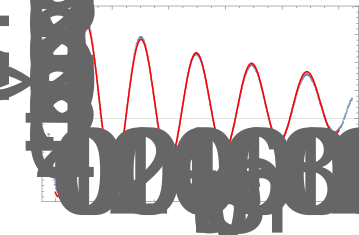
\includegraphics[width=8cm]{figs/drivenplot.png}
\caption{Driven Oscillations: $\beta = 0.001166$, $\omega = 0.03221$, $\delta=-0.04917$}
\label{fig:driven}
\end{figure}

\begin{figure}[b]
\centering
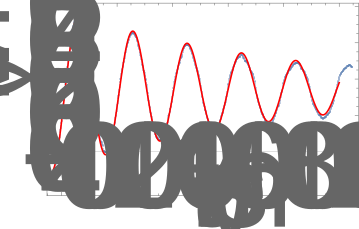
\includegraphics[width=8cm]{figs/counterclockwise2plot.png}
\caption{Counterclockwise Oscillations Trial 2: $\beta = 0.001199$, $\omega = 0.03212$, $\delta=-0.03436$}
\end{figure}

\begin{figure}[t]
\centering
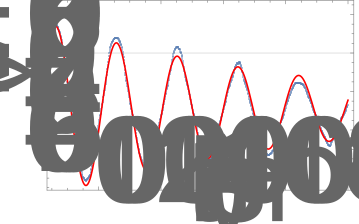
\includegraphics[width=8cm]{figs/clockwise1plot.png}
\caption{Clockwise Oscillations Trial 1: $\beta = 0.001130$, $\omega = 0.03222$, $\delta=0.02973$}
\end{figure}

\begin{figure}
\centering
\includegraphics[width=8cm]{figs/calibration.png}
\caption{Calibration Fit: $K=-\SI{38.1552}{mV \per \radian}$, $C=\SI{0.8320}{mV}$}
\label{fig:calibration}
\end{figure} 

Using the voltage data from the driven oscillations, we calibrate the
device by comparing the maximal and minimal values of $V$ with the
corresponding values of $\theta$ obtained by observing the change in the
position of the reflected laser beam. The relation between these two
variables is linear, given by $V = K \theta + C$, where $K$
and $C$ are fitting parameters (see figure~\ref{fig:calibration}).

To determine the torsional constant $\lambda$, we use the fact that the
period of oscillation is dependent on $\lambda$ by the equation
\[
    T = 2\pi \sqrt{I \over \lambda}.
\]
Rearranging gives
\[
    \lambda = I \left(\frac{2\pi}{T}\right)^2 = I \omega_0^2,
\]
where $\omega_0$ is the natural frequency of oscillation. From the fitting
parameter, we know the damping coefficient $\beta$ and the angular
frequency $\omega$, where
\[
    \omega^2 = \omega_0^2 - \beta^2.
\]
Thus, we find the natural frequency from the fit parameters to be
\[
    \omega_0^2 = \omega^2 + \beta^2.    
\]

We experimentally determined that $\omega_0 =
\SI{32.23e-3}{\radian\per\second}$ and $\beta = \SI{1.223e-3}{\per
\second}$. Using~\eqref{eq:moment_of_inertia} we find
\[
    I = \SI{1.403e-4}{kg.m^2}
\]
and therefore we have that
\[
    \lambda = \SI{1.457e-7}{N.m/\radian}.
\]
From~\eqref{eq:voltage_fit}, we can determine the voltage at equilibrium is
simply the fitting parameter $\delta$. Moreover, we can find the equilibrium
angle to be
\[
    \theta = \frac{\delta - C}{K}.
\]
We determine $\theta_1$, the equilibrium angle in the counterclockwise
setup, as well as $\theta_2$, the equilibrium angle in the clockwise setup.
The angle $\theta_0$ is obtained by taking the average of $\theta_1$ and
$\theta_2$, that is
\[
    \theta_0 = \frac{1}{2}(\theta_1 + \theta_2).
\]
We find that $\theta_1 = \SI{0.0226}{\radian} \approx
\SI{1.294}{\degree}$, $\theta_2 = \SI{0.0209}{\radian} \approx
\SI{1.198}{\degree}$, and $\theta_0 = \SI{0.0217}{\radian} \approx
\SI{1.246}{\degree}$.

It is now possible to calculate $G$. We find two separate values: one for
the counterclockwise setup, $G_1$, and one for the clockwise setup, $G_2$.
Using equation~\eqref{eq:gravitational_constant}, we find
\[
    G_1 = \SI{7.485e-11}{N.\meter^2 \per \kilogram^2}
\]
and
\[
    G_2 = \SI{7.523e-11}{N.m^2/kg^2}.
\]  
Taking the average of $G_1$ and $G_2$, we calculate the value of the
gravitational constant to be
\[
    G = \SI{7.504e-11}{N.m^2/kg^2}.
\]
There are many errors associated with this measurement, which will be
discussed in the next section.

\section{Error}
We first determine a systematic error on our measurement of $G$. From
equation~\eqref{eq:gravitational_constant}, we can see that $G$ is a
function of the variables $m$, $M$, $b$, $d$, $\theta_0$, $\theta_1$,
$\theta_2$, $\rho$, $I$, and $L$. For convenience, we will simply say that
$G = G(x_1,\ldots,x_{10})$, where each $x_i$ is one of the variables listed
above. Assuming the variables are independent, the standard deviation on our
measurement of $G$ is given by
\[
    \sigma_G = \sqrt{\sum_{j=1}^{10} \left( \frac{\d G}{\d x_j} \right)^2
    \sigma_{x_j}^2}.
\]
For the known quantities, including the mass of the tungsten spheres and
the mass density of the rod, we assumed no uncertainty. Additionally, we
assume that the error in our measurement of $\theta_0$ is within one
thousandth of a degree, or about $\SI{1.75e-5}{\radian}$. This error
accounts for possible asymmetries in the experimental setup. The standard
deviation of the measurement of $G$ is found numerically to be
\[
    \sigma_G = \SI{1.431e-11}{Nm^2/kg^2}.
\]
As mentioned previously, we assumed that there was no uncertainty in the
values of the ``known'' quantities. Recalculating $\sigma_G$ with small
($1\%$) uncertainties in these quantities produces a negligible affect on
the uncertainty of $G$. Thus, the calculated value of $\sigma_G$ shown
above is sufficiently accurate.

\section{Conclusion}

We were able to calculate the value of $G$ to be
\[
    G = (7.501 \pm 1.431)\times 10^{-11} \,\si{N.m^2/kg^2}.
\]
Comparing this with the known of $G$, $G_0 = \SI{6.67e-11}{N.m^2/kg^2}$, we can
see that $G_0$ falls within one standard deviation of our measurement.
Thus, our experimentally determined value of $G$ agrees reasonably with the
known value. 

\end{document}
